% This file was created with tikzplotlib v0.10.1.
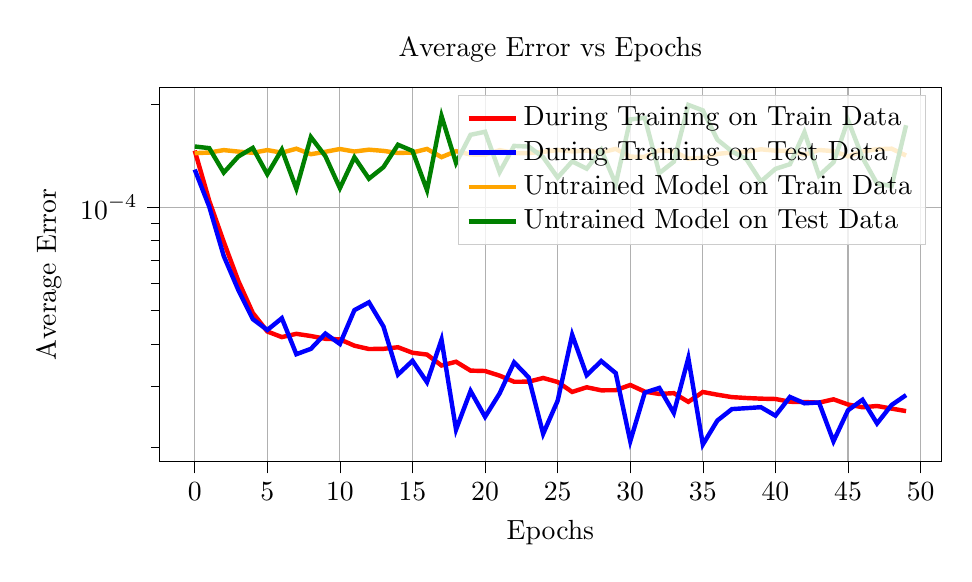
\begin{tikzpicture}

    \definecolor{darkgray176}{RGB}{176,176,176}
    \definecolor{green}{RGB}{0,128,0}
    \definecolor{lightgray204}{RGB}{204,204,204}
    \definecolor{orange}{RGB}{255,165,0}
    
    \begin{axis}[
      width = 0.95\textwidth,
      height = 18em,
    legend cell align={left},
    legend style={
      fill opacity=0.8,
      draw opacity=1,
      text opacity=1,
      % at={(0.91,0.5)},
      % anchor=east,
      draw=lightgray204
    },
    % log basis y={10},
    tick align=outside,
    tick pos=left,
    title={Average Error vs Epochs},
    x grid style={darkgray176},
    xlabel={Epochs},
    xmajorgrids,
    xmin=-2.45, xmax=51.45,
    xtick style={color=black},
    y grid style={darkgray176},
    ylabel={Average Error},
    ymajorgrids,
    ymin=1.81602095355054e-05, ymax=0.000222783350611656,
    ymode=log,
    ytick style={color=black},
    ytick={1e-06,1e-05,0.0001,0.001,0.01},
    yticklabels={
      \(\displaystyle {10^{-6}}\),
      \(\displaystyle {10^{-5}}\),
      \(\displaystyle {10^{-4}}\),
      \(\displaystyle {10^{-3}}\),
      \(\displaystyle {10^{-2}}\)
    }
    ]
    \addplot [ultra thick, red]
    table {%
    0 0.000146278194733895
    1 0.000104420905699953
    2 7.92681239545345e-05
    3 6.10758288530633e-05
    4 4.92224680783693e-05
    5 4.34550092904828e-05
    6 4.18473209720105e-05
    7 4.27740997110959e-05
    8 4.21492586610839e-05
    9 4.13740053772926e-05
    10 4.12062763643917e-05
    11 3.95096503780223e-05
    12 3.86323808925226e-05
    13 3.8685386243742e-05
    14 3.90951099689119e-05
    15 3.7674093618989e-05
    16 3.72231625078712e-05
    17 3.45841617672704e-05
    18 3.54710755345877e-05
    19 3.34202304657083e-05
    20 3.33290299749933e-05
    21 3.23112872138154e-05
    22 3.10100913338829e-05
    23 3.1028324883664e-05
    24 3.18035745294765e-05
    25 3.09636925521772e-05
    26 2.89666477328865e-05
    27 2.98817540169694e-05
    28 2.92815784632694e-05
    29 2.92987824650481e-05
    30 3.03483375319047e-05
    31 2.90223379124654e-05
    32 2.85742298729019e-05
    33 2.87294860754628e-05
    34 2.71037642960437e-05
    35 2.89524341496872e-05
    36 2.84268226096174e-05
    37 2.79751275229501e-05
    38 2.78087027254514e-05
    39 2.76841983577469e-05
    40 2.76240880339174e-05
    41 2.71164917649003e-05
    42 2.70670807367424e-05
    43 2.69537595158909e-05
    44 2.75629245152231e-05
    45 2.6622759833117e-05
    46 2.61352506640833e-05
    47 2.63559304585215e-05
    48 2.59002445091028e-05
    49 2.54677142947912e-05
    };
    \addlegendentry{During Training on Train Data}
    \addplot [ultra thick, blue]
    table {%
    0 0.000128779443912208
    1 0.00010038409527624
    2 7.20859316061251e-05
    3 5.74429686821532e-05
    4 4.72210740554146e-05
    5 4.38880924775731e-05
    6 4.74986336485017e-05
    7 3.7310368497856e-05
    8 3.86739084206056e-05
    9 4.2848852899624e-05
    10 3.9968599594431e-05
    11 5.0143735279562e-05
    12 5.285011138767e-05
    13 4.49300969194155e-05
    14 3.25484543282073e-05
    15 3.56887139787432e-05
    16 3.09173701680265e-05
    17 4.11355395044666e-05
    18 2.24964205699507e-05
    19 2.91467531496892e-05
    20 2.45067039941205e-05
    21 2.86695176328067e-05
    22 3.53258474206086e-05
    23 3.19383507303428e-05
    24 2.18671866605291e-05
    25 2.73038804152748e-05
    26 4.2485826270422e-05
    27 3.24111788359005e-05
    28 3.56320124410558e-05
    29 3.28617716149893e-05
    30 2.08107903745258e-05
    31 2.8820493753301e-05
    32 2.97523602057481e-05
    33 2.5161634766846e-05
    34 3.63602011930197e-05
    35 2.03521376533899e-05
    36 2.3903059627628e-05
    37 2.58119016507408e-05
    38 2.59747375821462e-05
    39 2.61434706771979e-05
    40 2.47025800490519e-05
    41 2.80039475910598e-05
    42 2.68369312834693e-05
    43 2.69887150352588e-05
    44 2.07989851332968e-05
    45 2.56072144111386e-05
    46 2.74763297056779e-05
    47 2.34442468354246e-05
    48 2.65273101831554e-05
    49 2.83582612610189e-05
    };
    \addlegendentry{During Training on Test Data}
    \addplot [ultra thick, orange]
    table {%
    0 0.000143817727803253
    1 0.000144362973514944
    2 0.000146766687976196
    3 0.000145289624924771
    4 0.000144115459988825
    5 0.000146782738738693
    6 0.000144232981256209
    7 0.000148136517964303
    8 0.000142785676871426
    9 0.000145113124744967
    10 0.000147847051266581
    11 0.000145348269143142
    12 0.000147180369822308
    13 0.000145986239658669
    14 0.000143930912599899
    15 0.000144404504681006
    16 0.000147901533637196
    17 0.000139990574098192
    18 0.000145746729685925
    19 0.000142500211950392
    20 0.000142163597047329
    21 0.000146696082083508
    22 0.00014386406110134
    23 0.000143894605571404
    24 0.000145068916026503
    25 0.000146825681440532
    26 0.000145544589031488
    27 0.000146261707413942
    28 0.000144508856465109
    29 0.000147926708450541
    30 0.000140387055580504
    31 0.000140381875098683
    32 0.00014663758338429
    33 0.00014546888996847
    34 0.000138474060804583
    35 0.000139353855047375
    36 0.000143018041853793
    37 0.000144513905979693
    38 0.000145408208481967
    39 0.00014754910080228
    40 0.000146216785651632
    41 0.000146020873216912
    42 0.000142244753078558
    43 0.000146861115354113
    44 0.000145769605296664
    45 0.000140737523906864
    46 0.000145486628753133
    47 0.000147612619912252
    48 0.000148156919749454
    49 0.000141483877087012
    };
    \addlegendentry{Untrained Model on Train Data}
    \addplot [ultra thick, green]
    table {%
    0 0.000150364750879817
    1 0.000148715800605714
    2 0.000126212136819959
    3 0.000140571341034956
    4 0.00014891754835844
    5 0.0001248148328159
    6 0.000147257611388341
    7 0.000113281806989107
    8 0.000160188879817724
    9 0.000140890551847406
    10 0.000113709320430644
    11 0.000139861251227558
    12 0.00012114318087697
    13 0.000130904605612159
    14 0.000152134743984789
    15 0.000145973521284759
    16 0.000112183719465975
    17 0.000184424745384604
    18 0.000134632413391955
    19 0.00016261384007521
    20 0.000165981182362884
    21 0.00012655348109547
    22 0.000150970416143537
    23 0.000150248713907786
    24 0.000139949814183637
    25 0.000122067860502284
    26 0.000136034286697395
    27 0.000129538966575637
    28 0.000146950769703835
    29 0.000116940143925603
    30 0.000180271337740123
    31 0.000182227056939155
    32 0.000125736318295822
    33 0.000135748166940175
    34 0.000198789552086964
    35 0.000191611266927794
    36 0.000157448623212986
    37 0.000145551850437187
    38 0.000138119357870892
    39 0.000118853095045779
    40 0.000129383552120999
    41 0.000133493827888742
    42 0.00016541252261959
    43 0.000123607329442166
    44 0.000135195485199802
    45 0.000179384034709074
    46 0.000139412193675525
    47 0.00011720007751137
    48 0.000115313268906903
    49 0.000173394801095128
    };
    \addlegendentry{Untrained Model on Test Data}
    \end{axis}
    
    \end{tikzpicture}
    